% Manual template (AAT2), see docs/HowToDoc.md
% Build (in docs/manual):  pdflatex ManualYourPluginName.tex   (twice, for the references)
% The PDF is copied into the release zips by the GitHub workflow.
\documentclass[12pt]{article}
\usepackage[utf8]{inputenc}
\usepackage[T1]{fontenc}
\usepackage[top=2cm, bottom=2cm, left=2cm, right=2cm]{geometry}
\usepackage{graphicx}
\usepackage{xcolor}
\usepackage{hyperref}
\hypersetup{colorlinks=true, linkcolor=red, urlcolor=red, pdftitle={YourPluginName Documentation}}

% ---- change these ------------------------------------------------------------
\newcommand{\pluginversion}{0.0.1}   % the version in CMakeLists.txt
\newcommand{\pluginauthor}{YourName}
\newcommand{\sourceurl}{https://github.com/YourGitHubName/YourPluginName}
% -------------------------------------------------------------------------------

\title{YourPluginName Documentation}
\author{License: CC-BY 4.0}
\date{\today, for YourPluginName \pluginversion}

\begin{document}
\maketitle

\section{Introduction}
What does YourPluginName do, and what is it good for? Two or three sentences for someone who
has never seen it. Then, if needed, a warning (e.g. about loud sounds) and a personal note.

\section{Installation}
The downloaded file is a zip file. It contains the plug-in (.vst3; on macOS also the AU,
.component), the Standalone application, a ReadMeFirst.txt, the licence files and this manual.
Copy the plug-in to the right place and let your DAW rescan its plug-ins.

\begin{verbatim}
Windows (VST3):  C:\Program Files\Common Files\VST3
Mac (VST3):      /Users/yourUSERNAME/Library/Audio/Plug-Ins/VST3
Mac (AU):        /Users/yourUSERNAME/Library/Audio/Plug-Ins/Components
Linux (VST3):    /home/yourUSERNAME/.vst3
\end{verbatim}

The macOS version is not signed with an Apple Developer ID. If macOS reports that the plug-in
is damaged or cannot be opened, remove the quarantine flag in the Terminal, e.g.
\texttt{xattr -cr \textasciitilde/Library/Audio/Plug-Ins/VST3/YourPluginName.vst3}.

\subsection{Presets and settings}
The presets (plain XML files) and the settings file (\texttt{user.settings}: day/night theme)
are stored in this folder -- delete it to remove YourPluginName completely:
\begin{verbatim}
Windows: C:\Users\yourUSERNAME\AppData\Roaming\YourCompany\YourPluginName
Mac:     /Users/yourUSERNAME/Library/Audio/Presets/YourCompany/YourPluginName
Linux:   /home/yourUSERNAME/.config/YourCompany/YourPluginName
\end{verbatim}

\section{How to use}
\begin{center}
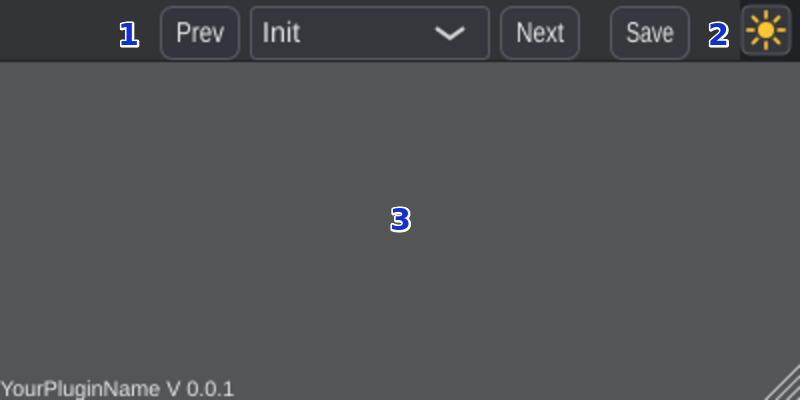
\includegraphics[width=0.8\textwidth]{images/GUI_Numbers.png}
\end{center}
\begin{enumerate}
    \item \textbf{Preset handler}: Prev/Next step through the presets. To save a new preset,
    type a name and press Save. Save turns red when you change a parameter of the displayed
    preset; press it to update the preset. To delete a preset, delete its XML file.
    \item \textbf{Day/night}: switches between the night (dark) and the day (light) theme.
    \item \textbf{Your controls}: describe the parts of your GUI here (see section~\ref{sec:controls}
    for the list of all controls).
\end{enumerate}

\section{Controls}\label{sec:controls}
All controls, their range and default value. Rest the mouse on a control to see its
description as a tooltip.

\begin{center}
\small
% generated from the code: YourPluginName_Tester --manual tex > controls.tex (see docs/HowToDoc.md)
\begin{tabular}{p{0.2\textwidth}p{0.22\textwidth}p{0.12\textwidth}p{0.36\textwidth}}
\hline
Control & Range & Default & Description \\
\hline
Example & 1.0 xyz - 2.0 xyz & 1.2 xyz & An example parameter; replace it with your own. \\
\hline
\end{tabular}

\end{center}

\section{How it works}
Optional: the idea behind the algorithm, in a few sentences and maybe a block diagram.

\section{Source code}
YourPluginName is open source. You find the source code here:\newline
\url{\sourceurl}. Please report bugs there, too.

\section{Legal stuff}
For this documentation the CC-BY 4.0 licence is valid. Copyright holder is \pluginauthor.
The source code of the plug-in is under the MIT licence. The plug-in binaries contain JUCE
(used under the AGPLv3), the VST3 SDK (MIT) and, on macOS, the Audio Unit SDK (Apache 2.0);
the binaries as a whole are distributed under the AGPLv3.

\begin{itemize}
    \item Microsoft\textsuperscript{\textregistered}, Windows\textsuperscript{\textregistered}
    are trademarks of the Microsoft group of companies.
    \item Mac\textsuperscript{\textregistered} is a trademark of Apple Inc.
    \item VST\textsuperscript{\textregistered} is a registered trademark of Steinberg Media
    Technologies GmbH.
\end{itemize}

\end{document}
